\let\negmedspace\undefined
\let\negthickspace\undefined
\documentclass[journal]{IEEEtran}
\usepackage[a5paper, margin=10mm, onecolumn]{geometry}
%\usepackage{lmodern} % Ensure lmodern is loaded for pdflatex
\usepackage{tfrupee} % Include tfrupee package

\setlength{\headheight}{1cm} % Set the height of the header box
\setlength{\headsep}{0mm}     % Set the distance between the header box and the top of the text

\usepackage{gvv-book}
\usepackage{gvv}
\usepackage{cite}
\usepackage{amsmath,amssymb,amsfonts,amsthm}
\usepackage{algorithmic}
\usepackage{graphicx}
\usepackage{textcomp}
\usepackage{xcolor}
\usepackage{txfonts}
\usepackage{listings}
\usepackage{enumitem}
\usepackage{mathtools}
\usepackage{gensymb}
\usepackage{comment}
\usepackage[breaklinks=true]{hyperref}
\usepackage{tkz-euclide} 
\usepackage{listings}
% \usepackage{gvv}                                        
\def\inputGnumericTable{}                                 
\usepackage[latin1]{inputenc}                                
\usepackage{color}                                            
\usepackage{array}                                            
\usepackage{longtable}                                       
\usepackage{calc}                                             
\usepackage{multirow}                                         
\usepackage{hhline}                                           
\usepackage{ifthen}                                           
\usepackage{lscape}
\begin{document}

\bibliographystyle{IEEEtran}
\vspace{3cm}

\title{5.2.9}
\author{EE25BTECH11006 - ADUDOTLA SRIVIDYA}
% \maketitle
% \newpage
% \bigskip
{\let\newpage\relax\maketitle}

\renewcommand{\thefigure}{\theenumi}
\renewcommand{\thetable}{\theenumi}
\setlength{\intextsep}{10pt}


\textbf{Question:}
Solve the simultaneous linear equations
$5u-4v+8=0$ , $7u+6v-9=0$.

\textbf{Solution:}\\
\begin{align}
5u - 4v &= -8 
\end{align}
\begin{align}
7u + 6v &= 9
\end{align}

\begin{align}
\myvec{5 & -4 \\ 7 & 6}\myvec{u \\ v}=\myvec{-8 \\ 9}
\end{align}

Augmented matrix,
\begin{align}
\myvec{5 & -4 & -8 \\ 7 & 6 & 9} 
\end{align}

\begin{align}
\myvec{5 & -4 & -8 \\ 7 & 6 & 9}
\xrightarrow{R_2 \rightarrow 5R_2-7R_1}
\myvec{5 & -4 & -8 \\ 0 & 58 & 101}
\xrightarrow{R_2 \rightarrow \dfrac{r_2}{58}}
\myvec{5 & -4 & -8 \\ 0 & 1 & \dfrac{101}{58}}
\end{align}
\begin{align}
\myvec{5 & -4 & -8 \\ 0 & 1 & \dfrac{101}{58}}
\xrightarrow{R_1 \rightarrow R_1+4R_2}
\myvec{5 & 0 & -\dfrac{30}{29} \\ 0 & 1 & \dfrac{101}{58}}
\xrightarrow{R_1 \rightarrow \dfrac{R_1}{5}}
\myvec{1 & 0 & -\dfrac{6}{29} \\ 0 & 1 & \dfrac{101}{58}}
\end{align}


Thus, the solution vector is
\begin{align}
    \myvec{u \\ v}=\myvec{-\dfrac{6}{29} \\ \dfrac{101}{58}}
\end{align}

\newpage
\begin{figure}[H]
  \centering
  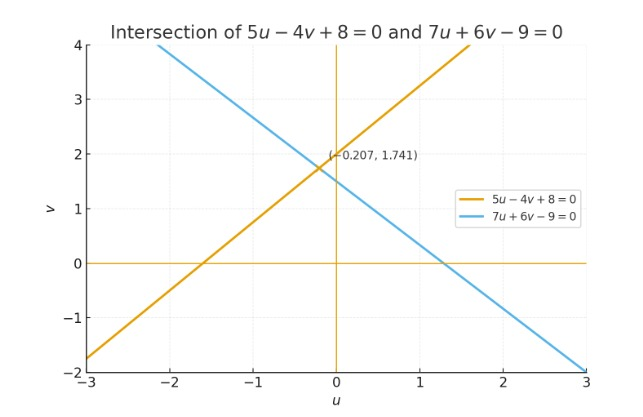
\includegraphics[width=0.8\linewidth]{figs/fig.jpeg}
  \caption{Intersection of $5u-4v+8=0$ and $7u+6v-9=0$ at
           $\left(-\tfrac{6}{29},\,\tfrac{101}{58}\right)$.}
  \label{fig:5.2.2}
\end{figure}





 

\end{document}
